\subsection{Baselines}
\label{sec:baselines}

\begin{figure}[tp]
    \vspace*{-\figskipabove px}
    \vspace{4px}
    \centering
    {\scriptsize
        
    \begin{subfigure}[t]{0.5\textwidth}
        \vspace{0px}\centering
	    \begin{subfigure}[t]{0.15\textwidth}
   	    	\vspace{0px}\centering
   	    	GT,\\High\\
	        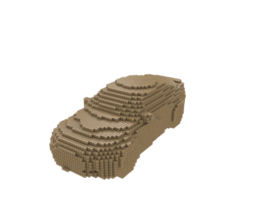
\includegraphics[width=1.5cm,trim={\cropleft cm \croplower cm \cropright cm \cropupper cm},clip]{gdat_shapenet_clean_high_0_bin_only}
	    \end{subfigure}
	    \begin{subfigure}[t]{0.15\textwidth}
   	    	\vspace{0px}\centering
   	    	GT\\
   	    	~\\
	        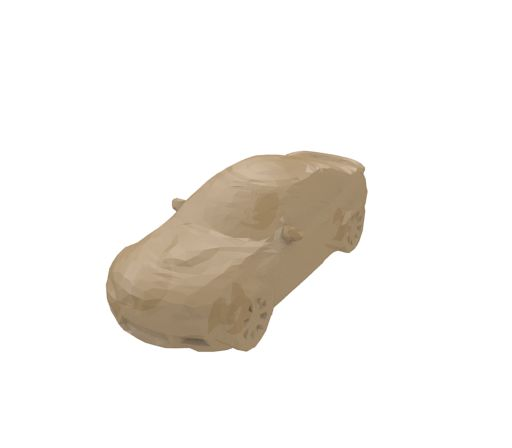
\includegraphics[width=1.5cm,trim={\cropleft cm \croplower cm \cropright cm \cropupper cm},clip]{gdat_shapenet_clean_low_0_gt_only}
	    \end{subfigure}
	    \begin{subfigure}[t]{0.15\textwidth}
   	    	\vspace{0px}\centering
   	    	\DVAE, Low\\
	        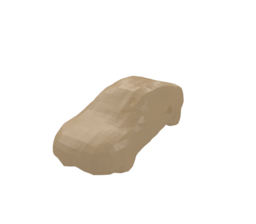
\includegraphics[width=1.5cm,trim={\cropleft cm \croplower cm \cropright cm \cropupper cm},clip]{gexp_clean_low_10_wide_prior_3_2_res_0}
	    \end{subfigure}
	    \begin{subfigure}[t]{0.15\textwidth}
   	    	\vspace{0px}\centering
   	    	\DVAE, High\\
   	    	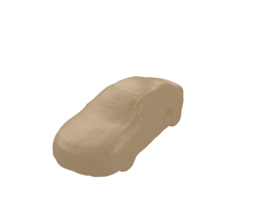
\includegraphics[width=1.5cm,trim={\cropleft cm \croplower cm \cropright cm \cropupper cm},clip]{gexp_clean_high_10_wide_prior_3_2_res_0}
	    \end{subfigure}
	    \begin{subfigure}[t]{0.15\textwidth}
   	    	\vspace{0px}\centering
   	    	\DVAE, Low\\
	        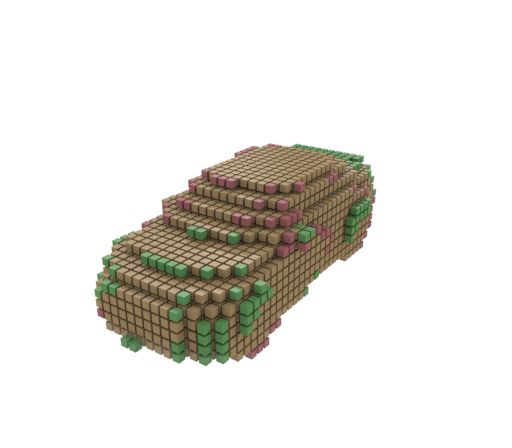
\includegraphics[width=1.5cm,trim={\cropleft cm \croplower cm \cropright cm \cropupper cm},clip]{gexp_clean_low_10_wide_prior_3_3_res_0}
	    \end{subfigure}
	    \begin{subfigure}[t]{0.15\textwidth}
   	    	\vspace{0px}\centering
   	    	\DVAE, High\\
	        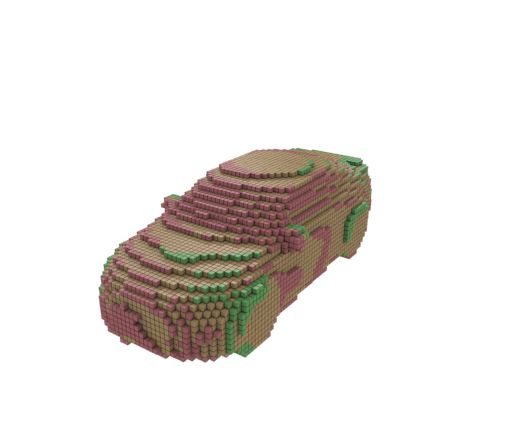
\includegraphics[width=1.5cm,trim={\cropleft cm \croplower cm \cropright cm \cropupper cm},clip]{gexp_clean_high_10_wide_prior_3_3_res_0}
	    \end{subfigure}
	    \\ %[-4px]
	    %\begin{subfigure}[t]{0.105\textwidth}
	    %	\vspace{0px}\centering
	    %	\includegraphics[width=1.5cm,trim={\cropleft cm \croplower cm \cropright cm \cropupper cm},clip]{gdat_modelnet_chair_low_1188_bin_only}
	    %\end{subfigure}
	    \begin{subfigure}[t]{0.15\textwidth}
   	    	\vspace{0px}\centering
	        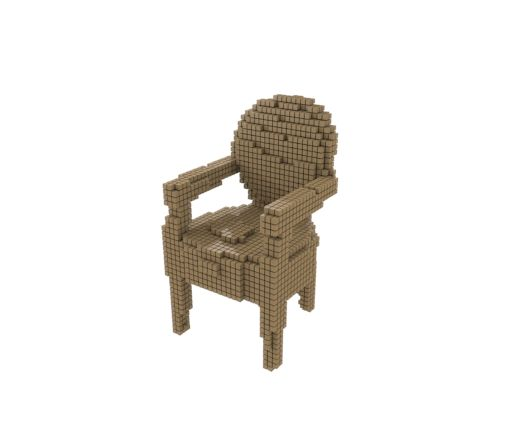
\includegraphics[width=1.5cm,trim={\cropleft cm \croplower cm \cropright cm \cropupper cm},clip]{gdat_modelnet_chair_high_1188_bin_only}
	    \end{subfigure}
	    \begin{subfigure}[t]{0.15\textwidth}
   	    	\vspace{0px}\centering
	        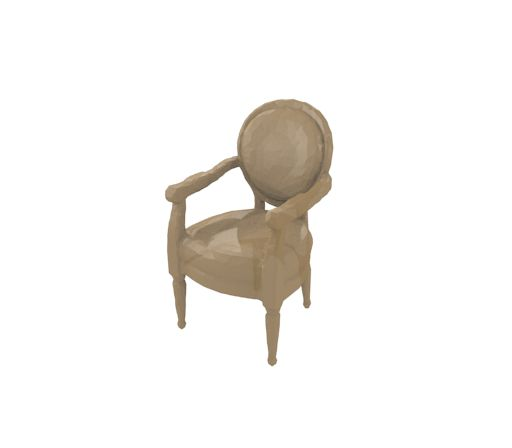
\includegraphics[width=1.5cm,trim={\cropleft cm \croplower cm \cropright cm \cropupper cm},clip]{gdat_modelnet_chair_low_1188_gt_only}
	    \end{subfigure}
	    \begin{subfigure}[t]{0.15\textwidth}
   	    	\vspace{0px}\centering
	        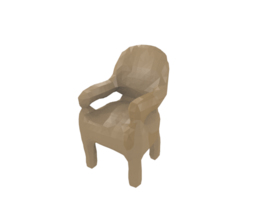
\includegraphics[width=1.5cm,trim={\cropleft cm \croplower cm \cropright cm \cropupper cm},clip]{gexp_clean_chair_low_10_wide_prior_3_2_res_1188}
	    \end{subfigure}
	    \begin{subfigure}[t]{0.15\textwidth}
   	    	\vspace{0px}\centering
   	    	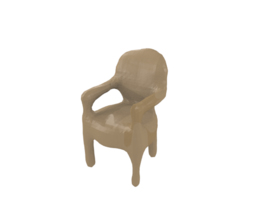
\includegraphics[width=1.5cm,trim={\cropleft cm \croplower cm \cropright cm \cropupper cm},clip]{gexp_clean_chair_high_10_wide_d_prior_3_2_res_1188}
	    \end{subfigure}
	    \begin{subfigure}[t]{0.15\textwidth}
   	    	\vspace{0px}\centering
	        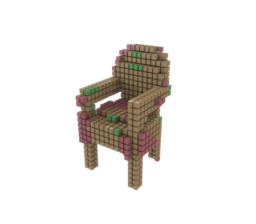
\includegraphics[width=1.5cm,trim={\cropleft cm \croplower cm \cropright cm \cropupper cm},clip]{gexp_clean_chair_low_10_wide_prior_3_3_res_1188}
	    \end{subfigure}
	    \begin{subfigure}[t]{0.15\textwidth}
   	    	\vspace{0px}\centering
	        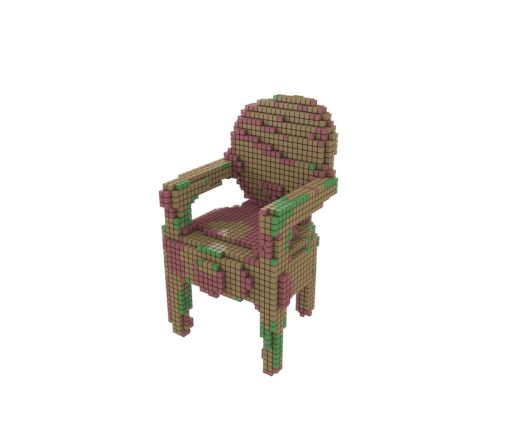
\includegraphics[width=1.5cm,trim={\cropleft cm \croplower cm \cropright cm \cropupper cm},clip]{gexp_clean_chair_high_10_wide_d_prior_3_3_res_1188}
	    \end{subfigure}
        \subcaption{Reconstructions, Low and High Resolution (\cf \tabref{tab:data})}
    \end{subfigure}
    \\[4px]
    \begin{subfigure}[t]{0.5\textwidth}
        \vspace{0px}\centering
	    \begin{subfigure}[t]{0.15\textwidth}
   	    	\vspace{0px}\centering
            Low\\
	        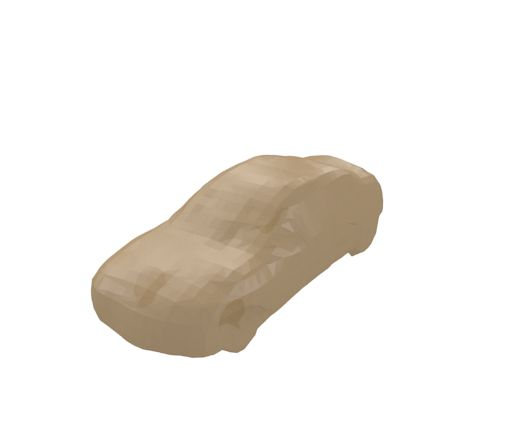
\includegraphics[width=1.5cm,trim={\cropleft cm \croplower cm \cropright cm \cropupper cm},clip]{gexp_clean_low_10_wide_prior_3_2_random_results_0}
	    \end{subfigure}
	    \begin{subfigure}[t]{0.15\textwidth}
   	    	\vspace{0px}\centering
            Low\\
	        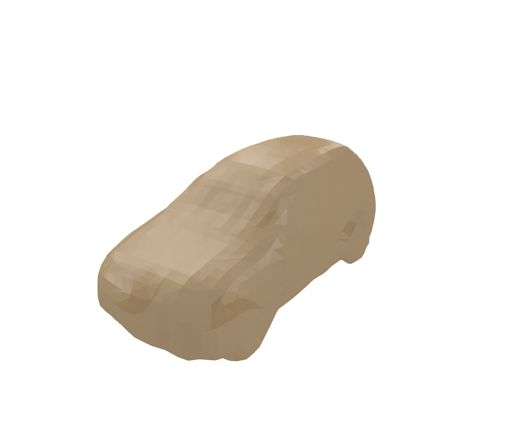
\includegraphics[width=1.5cm,trim={\cropleft cm \croplower cm \cropright cm \cropupper cm},clip]{gexp_clean_low_10_wide_prior_3_2_random_results_6}
	    \end{subfigure}
	    \begin{subfigure}[t]{0.15\textwidth}
   	    	\vspace{0px}\centering
            Low\\
	        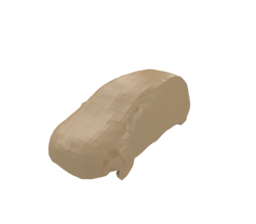
\includegraphics[width=1.5cm,trim={\cropleft cm \croplower cm \cropright cm \cropupper cm},clip]{gexp_clean_low_10_wide_prior_3_2_random_results_2}
	    \end{subfigure}
	    \begin{subfigure}[t]{0.15\textwidth}
   	    	\vspace{0px}\centering
            High\\
	        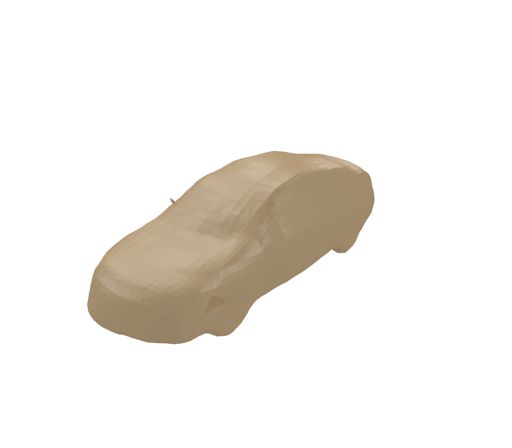
\includegraphics[width=1.5cm,trim={\cropleft cm \croplower cm \cropright cm \cropupper cm},clip]{gexp_clean_high_10_wide_prior_3_2_random_results_1}
	    \end{subfigure}
	    \begin{subfigure}[t]{0.15\textwidth}
   	    	\vspace{0px}\centering
            High\\
	        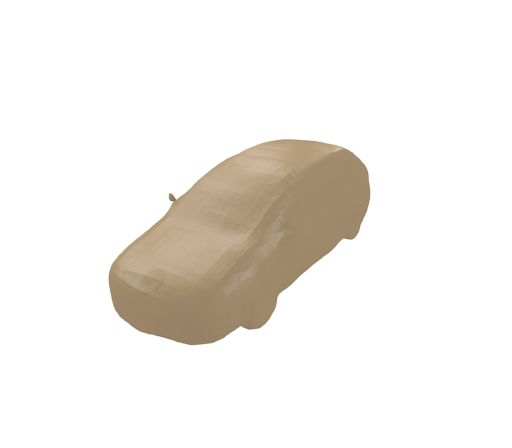
\includegraphics[width=1.5cm,trim={\cropleft cm \croplower cm \cropright cm \cropupper cm},clip]{gexp_clean_high_10_wide_prior_3_2_random_results_5}
	    \end{subfigure}
	    \begin{subfigure}[t]{0.15\textwidth}
   	    	\vspace{0px}\centering
            High\\
	        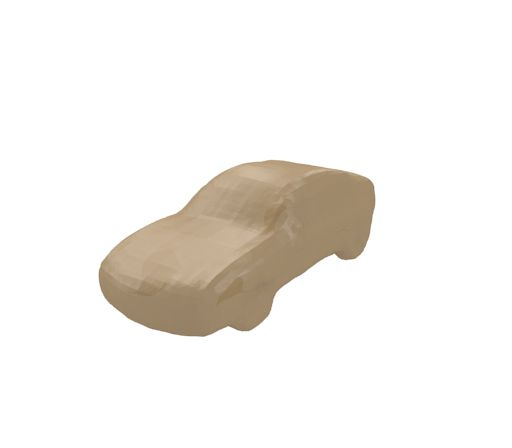
\includegraphics[width=1.5cm,trim={\cropleft cm \croplower cm \cropright cm \cropupper cm},clip]{gexp_clean_high_10_wide_prior_3_2_random_results_2}
	    \end{subfigure}
	    \\ %[-4px]
	    \begin{subfigure}[t]{0.15\textwidth}
   	    	\vspace{0px}\centering
   	       	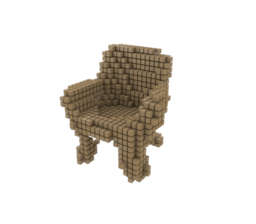
\includegraphics[width=1.5cm,trim={\cropleft cm \croplower cm \cropright cm \cropupper cm},clip]{gexp_clean_chair_low_10_wide_prior_3_3_random_results_1}
	    \end{subfigure}
	    \begin{subfigure}[t]{0.15\textwidth}
   	    	\vspace{0px}\centering
   	       	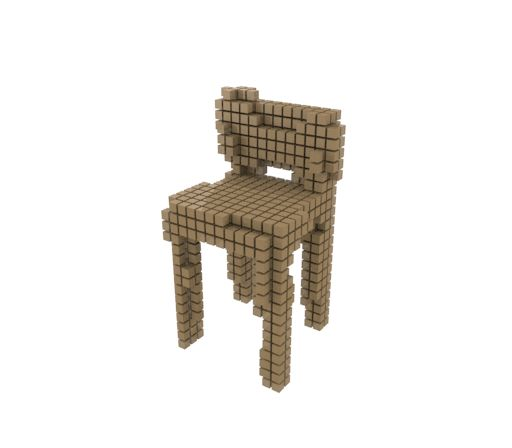
\includegraphics[width=1.5cm,trim={\cropleft cm \croplower cm \cropright cm \cropupper cm},clip]{gexp_clean_chair_low_10_wide_prior_3_3_random_results_6}
	    \end{subfigure}
	    \begin{subfigure}[t]{0.15\textwidth}
   	    	\vspace{0px}\centering
   	       	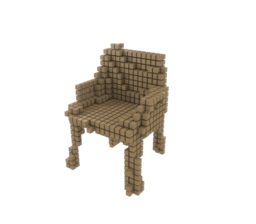
\includegraphics[width=1.5cm,trim={\cropleft cm \croplower cm \cropright cm \cropupper cm},clip]{gexp_clean_chair_low_10_wide_prior_3_3_random_results_2}
	    \end{subfigure}
	    \begin{subfigure}[t]{0.15\textwidth}
   	    	\vspace{0px}\centering
   	       	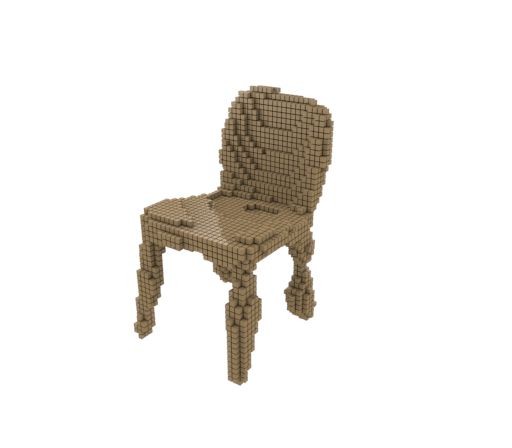
\includegraphics[width=1.5cm,trim={\cropleft cm \croplower cm \cropright cm \cropupper cm},clip]{gexp_clean_chair_high_10_wide_d_prior_3_3_random_results_1}
	    \end{subfigure}
	    \begin{subfigure}[t]{0.15\textwidth}
   	    	\vspace{0px}\centering
   	       	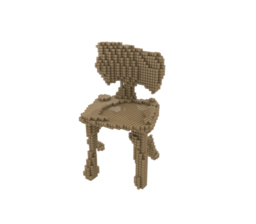
\includegraphics[width=1.5cm,trim={\cropleft cm \croplower cm \cropright cm \cropupper cm},clip]{gexp_clean_chair_high_10_wide_d_prior_3_3_random_results_0}
	    \end{subfigure}
	    \begin{subfigure}[t]{0.15\textwidth}
   	    	\vspace{0px}\centering
   	       	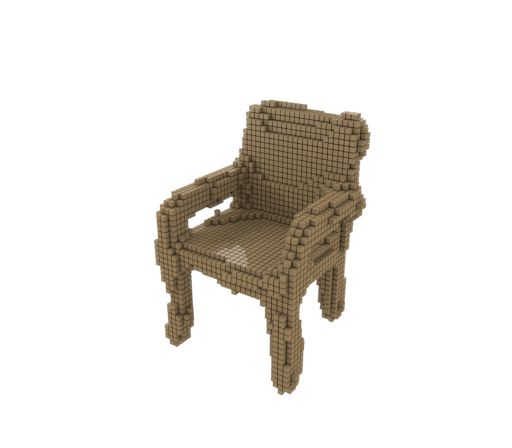
\includegraphics[width=1.5cm,trim={\cropleft cm \croplower cm \cropright cm \cropupper cm},clip]{gexp_clean_chair_high_10_wide_d_prior_3_3_random_results_3}
	    \end{subfigure}
        \subcaption{Random Samples, Low and High Resolution (\cf \tabref{tab:data})}
    \end{subfigure}
    }

    \vspace*{-\figskipcaption px}
    \caption{{\bf \DVAE Shape Prior.} Reconstructions and random samples on ShapeNet and ModelNet at multiple resolutions (\cf \tabref{tab:data}); false negative and false positive voxels in {\color{rgreen}green} and {\color{rred}red}. Our \DVAE shape prior provides high-quality reconstructions and meaningful random samples across resolutions.}
    \label{fig:results-shape-prior}
    \vspace*{-\figskipbelow px}
\end{figure}

\boldparagraph{Data-Driven Approaches}
%
{We consider the works by \cite{Engelmann2016GCPR} and \cite{Gupta2015CVPR} as data-driven baselines. Additionally, we consider regular maximum likelihood (\ML). \cite{Engelmann2016GCPR} -- referred to as \Engelmann\xspace-- use a principal component analysis shape prior trained on a manually selected set of car models\footnote{\url{https://github.com/VisualComputingInstitute/ShapePriors_GCPR16}}. Shape completion is posed as optimization problem considering both shape and pose. The pre-trained shape prior provided by Engelmann \etal assumes a ground plane which is, according to KITTI's LiDAR data, fixed at $1m$ height. Thus, we don't need to optimize pose on KITTI as we use the ground truth bounding boxes; on ShapeNet, in contrast, we need to optimize both pose and shape to deal with the random rotations in \clean and \noisy.}

Inspired by the work by \cite{Gupta2015CVPR} we also consider a shape retrieval and fitting baseline. Specifically, we perform iterative closest point (\ICP) \citep{Besl1992PAMI} fitting on all training shapes and subsequently select the best-fitting one. To this end, we uniformly sample $1\text{Mio}$ points on the training shapes, and perform point-to-point \ICP\footnote{\url{http://www.cvlibs.net/software/libicp/}.} for a maximum of $100$ iterations using $\left[\begin{matrix}R & t\end{matrix}\right] = \left[\begin{matrix}I_3 & 0\end{matrix}\right]$ as initialization. On the training set, we verified that this approach is always able to retrieve the perfect shape.

Finally, we consider a simple \ML baseline iteratively minimizing \eqnref{eq:ml} using stochastic gradient descent (SGD). This baseline is similar to the work by Engelmann \etal, however, like ours it is bound to the voxel grid. Per example, we allow a maximum of $5000$ iterations, starting with latent code $z = 0$, learning rate $0.05$ and momentum $0.5$ (decayed every $50$ iterations at rate $0.85$ and $1.0$ until $10^{-5}$ and $0.9$ have been reached).

\begin{figure}[tp]
    \vspace*{-\figskipabove px}
    \vspace{4px}
    \centering
    {\scriptsize
        
    \newcommand{\ablationa}{33}
    \newcommand{\ablationb}{99}
    \newcommand{\ablationc}{528}
    \newcommand{\ablationd}{693}
    \newcommand{\ablatione}{231}
    \newcommand{\ablationf}{396} % 396
    
    \begin{subfigure}[t]{0.01\textwidth}
        \vspace{0px}\centering
        \rotatebox[]{90}{\dAML\hspace*{0.25cm}}
    \end{subfigure}
    \begin{subfigure}[t]{0.07\textwidth}
        \vspace{0px}\centering
        \includegraphics[width=1.5cm,trim={\cropleft cm \croplower cm \cropright cm \cropupper cm},clip]{gexp_noisy_low_10_wide_w2_1_aml_3_2_res_\ablationa}
    \end{subfigure}
    \begin{subfigure}[t]{0.07\textwidth}
        \vspace{0px}\centering
        \includegraphics[width=1.5cm,trim={\cropleft cm \croplower cm \cropright cm \cropupper cm},clip]{gexp_noisy_low_10_wide_w2_1_aml_3_2_res_\ablationb}
    \end{subfigure}
    \begin{subfigure}[t]{0.07\textwidth}
        \vspace{0px}\centering
        \includegraphics[width=1.5cm,trim={\cropleft cm \croplower cm \cropright cm \cropupper cm},clip]{gexp_noisy_low_10_wide_w2_1_aml_3_2_res_\ablationc}
    \end{subfigure}
    \begin{subfigure}[t]{0.07\textwidth}
        \vspace{0px}\centering
        \includegraphics[width=1.5cm,trim={\cropleft cm \croplower cm \cropright cm \cropupper cm},clip]{gexp_noisy_low_10_wide_w2_1_aml_3_2_res_\ablationd}
    \end{subfigure}
    \begin{subfigure}[t]{0.07\textwidth}
        \vspace{0px}\centering
        \includegraphics[width=1.5cm,trim={\cropleft cm \croplower cm \cropright cm \cropupper cm},clip]{gexp_noisy_low_10_wide_w2_1_aml_3_2_res_\ablatione}
    \end{subfigure}
    \begin{subfigure}[t]{0.07\textwidth}
        \vspace{0px}\centering
        \includegraphics[width=1.5cm,trim={\cropleft cm \croplower cm \cropright cm \cropupper cm},clip]{gexp_noisy_low_10_wide_w2_1_aml_3_2_res_\ablationf}
    \end{subfigure}
    \\[-4px]
    \begin{subfigure}[t]{0.01\textwidth}
        \vspace{0px}\centering
        \rotatebox[]{90}{\AML\hspace*{0.25cm}}
    \end{subfigure}
    \begin{subfigure}[t]{0.07\textwidth}
        \vspace{0px}\centering
        \includegraphics[width=1.5cm,trim={\cropleft cm \croplower cm \cropright cm \cropupper cm},clip]{gexp_noisy_low_10_wide_w2_1_vae_aml_3_2_res_\ablationa}
    \end{subfigure}
    \begin{subfigure}[t]{0.07\textwidth}
        \vspace{0px}\centering
        \includegraphics[width=1.5cm,trim={\cropleft cm \croplower cm \cropright cm \cropupper cm},clip]{gexp_noisy_low_10_wide_w2_1_vae_aml_3_2_res_\ablationb}
    \end{subfigure}
    \begin{subfigure}[t]{0.07\textwidth}
        \vspace{0px}\centering
        \includegraphics[width=1.5cm,trim={\cropleft cm \croplower cm \cropright cm \cropupper cm},clip]{gexp_noisy_low_10_wide_w2_1_vae_aml_3_2_res_\ablationc}
    \end{subfigure}
    \begin{subfigure}[t]{0.07\textwidth}
        \vspace{0px}\centering
        \includegraphics[width=1.5cm,trim={\cropleft cm \croplower cm \cropright cm \cropupper cm},clip]{gexp_noisy_low_10_wide_w2_1_vae_aml_3_2_res_\ablationd}
    \end{subfigure}
    \begin{subfigure}[t]{0.07\textwidth}
        \vspace{0px}\centering
        \includegraphics[width=1.5cm,trim={\cropleft cm \croplower cm \cropright cm \cropupper cm},clip]{gexp_noisy_low_10_wide_w2_1_vae_aml_3_2_res_\ablatione}
    \end{subfigure}
    \begin{subfigure}[t]{0.07\textwidth}
        \vspace{0px}\centering
        \includegraphics[width=1.5cm,trim={\cropleft cm \croplower cm \cropright cm \cropupper cm},clip]{gexp_noisy_low_10_wide_w2_1_vae_aml_3_2_res_\ablationf}
    \end{subfigure}
    }
    \vspace*{-\figskipcaption px}
    \caption{{\bf Comparison of \AML and \dAML.} Our deterministic variant, \dAML, suffers from inferior results. Predicted shapes in {\color{rbeige}beige} and observations in {\color{rred}red} at low resolution ($24\ntimes54\ntimes24$ voxels).}
    \label{fig:results-shape-prior}
    \vspace*{-\figskipbelow px}
\end{figure}

\boldparagraph{Learning-Based Approaches}
%
Learning-based approaches usually employ an encoder-decoder architecture to directly learn a mapping from observations $x_n$ to ground truth shapes $y_n^*$ in a fully supervised setting \citep{Wang2017ICCV,Varley2017IROS,Yang2018ARXIVb,Yang2017ARXIV,Dai2017CVPRa}. While existing architectures differ slightly, they usually rely on a U-net architecture \citep{Ronneberger2015MICCAI,Cicek2016ARXIV}. In this paper, we use the approach of \cite{Dai2017CVPRa}\footnote{
    We use \url{https://github.com/angeladai/cnncomplete}. On ModelNet we added one convolutional stage in the en- and decoder for larger resolutions; on ShapeNet and KITTI, we needed to adapt the convolutional strides to fit the corresponding resolutions.
} -- referred to as \Dai\xspace --
as a representative baseline for this class of approaches. In addition, we consider a custom learning-based baseline which uses the architecture of our \DVAE shape prior, \cf \figref{fig:architectures}. In contrast to \citep{Dai2017CVPRa}, this baseline is also limited by the low-dimensional ($Q = 10$) bottleneck as it does not use skip connections.